\chapter{Theoretical Analysis} \label{chap:theoretical_analysis}
\section{Constant Velocity}
If we set the velocity profile of the equilibrium flow to constant $v_0=\text{const}$, then Eq.(\ref{eq:polynomial-eigenvalue-problem}) becomes a simple boundary value problem with second order constant coefficients differential equation.

\begin{equation} \label{eq:constant_v_problem_dirichlet}
    \omega^2\tilde{v} + 2i\omega\pdv{\tilde{v}}{z} + (1-v_0^2)\pdv[2]{\tilde{v}}{z} = 0
    \quad
    \tilde{v}(-1) = \tilde{v}(1) = 0
\end{equation}

The solution to this problem is
\begin{equation} \label{eq:constant_v_solution_dirichlet}
    \tilde{v} = \exp\left(-\frac{i\omega}{v_0+1}\right)
\left[ \exp\left(i\omega\frac{z+1}{v_0+1}\right) - \exp\left(i\omega\frac{z+1}{v_0-1}\right) \right], \quad \omega=n\pi(1-v_0^2)/2 \in \mathbb{R}.
\end{equation}

This result tells us for constant velocity case, the flow in magnetic nozzle is stable regardless the velocity $v_0$. It is worth to mention $v_0=1$ is a singular point of this problem.

We will use this as a base case and check our experimental results. 

\begin{figure}[H]
	\centering
	\begin{subfigure}{0.5\textwidth}
		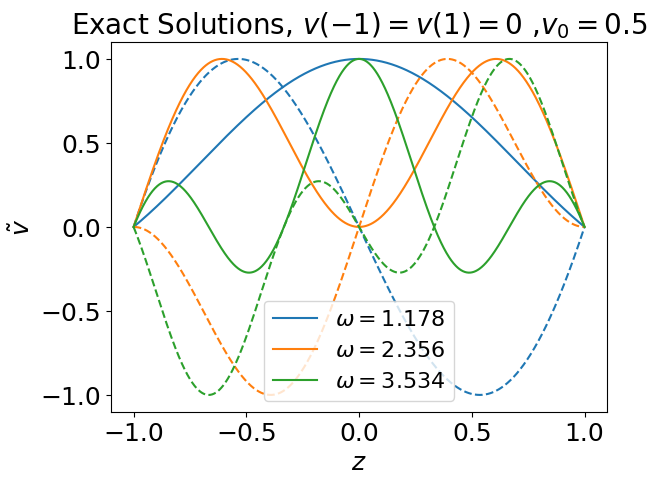
\includegraphics[width=\linewidth]{img/theoretical_analysis/exact_v0=0.5}
		\caption{Subsonic}
	\end{subfigure}%
	\begin{subfigure}{0.5\textwidth}
		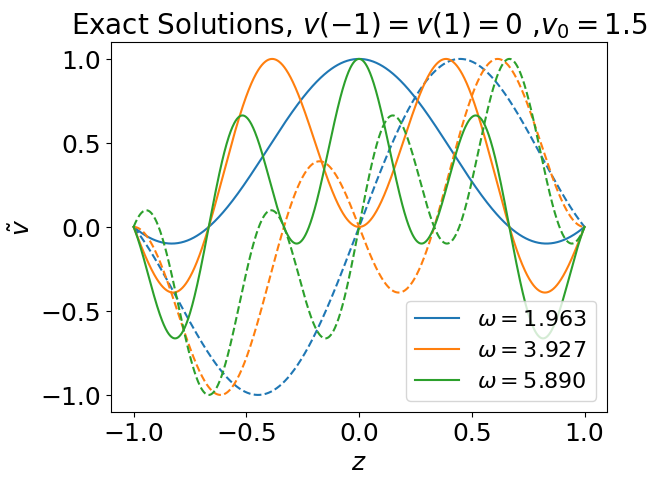
\includegraphics[width=\linewidth]{img/theoretical_analysis/exact_v0=1.5}
		\caption{Supersonic}
	\end{subfigure}
	\caption{The plots show the first three exact solutions to Eq.(\ref{eq:constant_v_problem_dirichlet}) for both subsonic and supersonic case. These solutions are stable.}
	\label{fig:exact_v}
\end{figure}

If we change the boundary condition to fixed left end and open right end, then we have the following problem
\begin{equation} \label{eq:constant_v_problem_openright}
    \omega^2\tilde{v} + 2i\omega\pdv{\tilde{v}}{z} + (1-v_0^2)\pdv[2]{\tilde{v}}{z} = 0
    \quad
    \tilde{v}(-1) = \pdv{\tilde{v}}{z}(1) = 0
\end{equation}
This is also easy to solve, the solution is 
\begin{equation} \label{eq:constant_v_solution_openright}
    v = \exp\left(-\frac{i\omega}{v_0+1}\right)\left[ \exp\left(i\omega\frac{z+1}{v_0+1}\right) - \exp\left(i\omega\frac{z+1}{v_0-1}\right) \right]
\end{equation} 
Depending on the value of $v_0$, the frequency $\omega$ can be real or complex,
\begin{equation}
    \begin{aligned}
        \omega &= (v_0^2-1) \left[ \frac{n\pi}{2} + \frac{1}{4}\cos^{-1}\left(\frac{v_0-1}{v_0+1}\right) \right] \in\mathbb{R}, \quad v_0>1 \\
        \omega &= (1-v_0^2) \left[ \frac{n\pi}{2} + \frac{1}{4}\cos^{-1}\left(\frac{v_0+1}{v_0-1}\right) \right] \in\mathbb{C}, \quad v_0<1
    \end{aligned}
\end{equation}
This tells us that the flow in magnetic nozzle with open right end is stable when $v_0>1$. For the case of $v_0<1$, since $\Im(\omega)<0$, so the oscillation is damped. Hence, the flow is also stable.

\begin{figure}[H]
	\centering
	\begin{subfigure}{0.5\textwidth}
		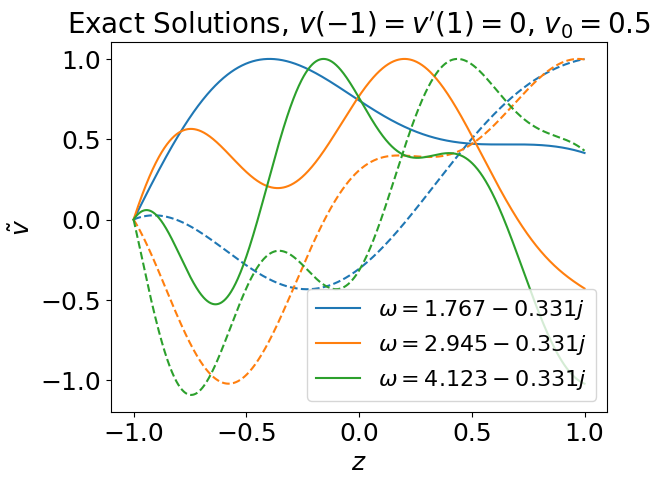
\includegraphics[width=\linewidth]{img/theoretical_analysis/exact_openright_v0=0.5}
		\caption{Subsonic}
	\end{subfigure}%
	\begin{subfigure}{0.5\textwidth}
		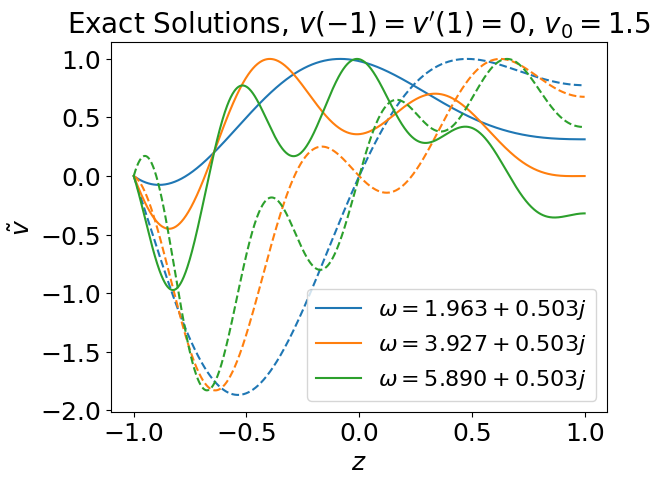
\includegraphics[width=\linewidth]{img/theoretical_analysis/exact_openright_v0=1.5}
		\caption{Supersonic}
	\end{subfigure}
	\caption{The plots show both subsonic and supersonic exact solutions to Eq.(\ref{eq:constant_v_problem_openright}). These solutions are stable.}
	\label{fig:exact_v_openright}
\end{figure}


\section{Spectral Pollution and Spurious Modes}
In this section, we will discuss an important phenomenon we will observe throughout the numerical experiments. It is the phenomenon of spectral pollution.

Spectral pollution refers to the phenomenon which some eigenvalues are not converging to the correct value when the mesh density is increased. When solving eigenvalue problems using spectral methods with finite difference or finite element approximations, spectral pollution might occur. \cite{llobet_spectral_1990}

\subsection{Finite Difference Discretization of Operators}
In this section, we are going to investigate the spectral pollution phenomenon when solving Eq.(\ref{eq:constant_v_problem_dirichlet}) using spectral method.

The dispersion relation can be obtained by substituting $\tilde{v} = \exp(-i\omega t + kx)$ into Eq.(\ref{eq:constant_v_problem_dirichlet}),
\begin{equation} \label{dispersion_relation}
	\omega = k(v_0 \pm 1) 
\end{equation}

If we assume $v\sim \exp(ikx)$, and let $\beta\equiv kh/2$. Then in finite difference discretization scheme, the differential operators $\dv*[n]{z}$ are equivalent to the following factors \cite{llobet_spectral_1990},
\begin{align}
	&G_0 = 1 \nonumber \\
	&G_1 = [\exp(2i\beta)-\exp(-2i\beta)]/2h = (i/h)\sin(2\beta) 
	\label{G-operator}\\
	&G_2 = [\exp(2i\beta)-2-\exp(-2i\beta)]/h^2 = (2/h^2)(\cos(2\beta)-1) \nonumber 
\end{align}


\subsection{Analysis of Numerical Spectrum}
\subsubsection{Discretize on the Same Grid}
Using the G-operator, Eq.(\ref{G-operator}), the discretized equation of Eq.(\ref{eq:constant_v_problem_dirichlet}) is 
\begin{equation} \label{eq:discretized_eq_G}
    (\omega^2G_0 + \omega G_1 + G_2)\mathbf{\tilde{v}} = 0
\end{equation}
where $\mathbf{\tilde{v}}$ is the discretized vector of $\tilde{v}$.

Solving Eq.(\ref{eq:discretized_eq_G}), we obtain the numerical dispersion relation,
\begin{equation} \label{dispersion_relation_G}
	\omega = \frac{2\sin(\beta)}{h}\left(v_0 \pm \sqrt{1 - v_0^2\sin[2](\beta)}\right)
\end{equation}

Given $h$ (fixed the mesh resolution), we see that
\begin{itemize}
	\item $\omega$ is real for all $k$ if $v_0 < 1$.
	\item $\omega$ is complex for large $k$, more specifically $k>h/2\arcsin(1/v_0)$, if $v_0 > 1$.
	\item For small $k$, meaning $k\to 0$, Eq.(\ref{dispersion_relation_G}) is a good representation for the analytical dispersion relation, Eq.(\ref{dispersion_relation}). 
\end{itemize}
This explains why the spurious unstable modes occur when $v_0>1$.

\begin{figure}[H]
	\centering
	\begin{subfigure}[b]{0.5\linewidth}
		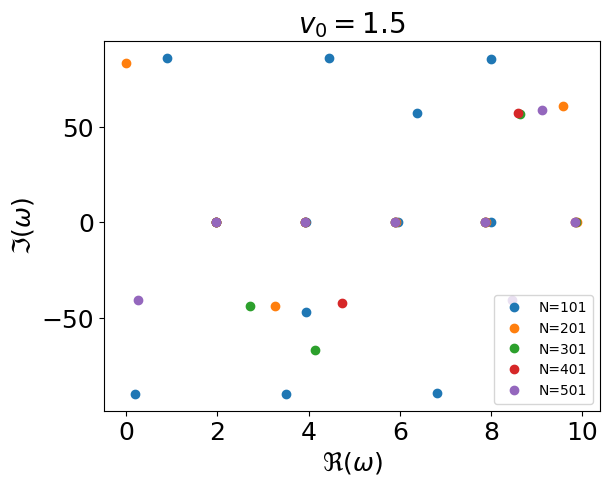
\includegraphics[width=\linewidth]{img/theoretical_analysis/eigvals_bad} 
		\caption{Bad eigenvalues}
	\end{subfigure}%
	\begin{subfigure}[b]{0.5\linewidth}
		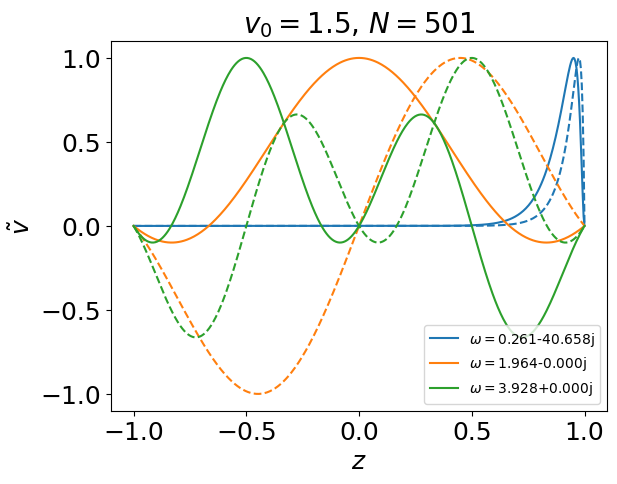
\includegraphics[width=\linewidth]{img/theoretical_analysis/eigvecs_bad} 
		\caption{Bad eigenfunctions}
	\end{subfigure}
	\caption{Spurious modes.}
	\label{fig:results_bad}
\end{figure}

One way to filter the spurious modes is to remove all modes with $k>h/2 \arcsin(1/v_0)$, see Fig.\ref{fig:results_filter_k}. However, this is not a good way to deal with general cases because it requires the solution to the discretized problem Eq.(\ref{eq:discretized_eq_G}). For general problem with non-constant velocity profile, it is hard to solve the discretized problem directly.

\begin{figure}[H]
	\centering
	\begin{subfigure}[b]{0.5\linewidth}
		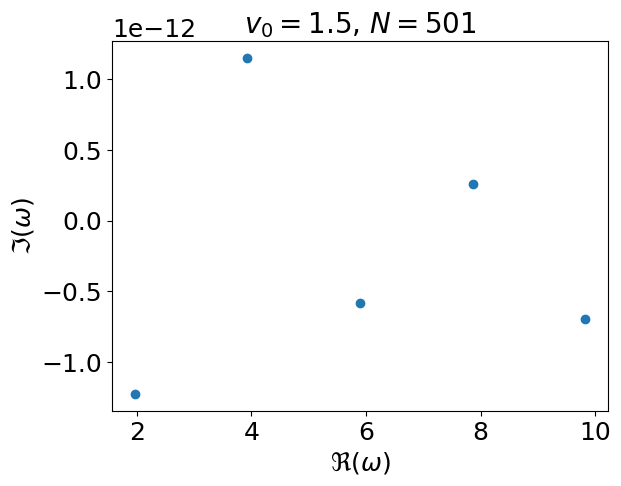
\includegraphics[width=\linewidth]{img/theoretical_analysis/eigvals_good} 
		\caption{Good eigenvalues}
	\end{subfigure}%
	\begin{subfigure}[b]{0.5\linewidth}
		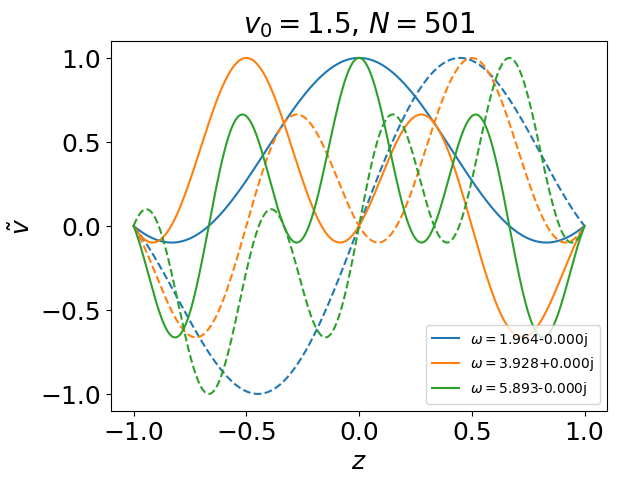
\includegraphics[width=\linewidth]{img/theoretical_analysis/eigvecs_good} 
		\caption{Good eigenfunctions}
	\end{subfigure}
	\caption{Filter out the spurious modes with $k>h/2\arcsin(1/v_0)$.}
	\label{fig:results_filter_k}
\end{figure}

A better way to filter the spurious modes is by doing a "convergence test". Since the frequency Eq.(\ref{dispersion_relation_G}) is changing with mesh resolution $h$. We can simply solve the discretized problem using spectral method under different mesh resolution. Then filter out the eigenmodes that are changing dramatically.